\documentclass{article}
\usepackage[utf8]{inputenc}
\usepackage[portuges]{babel}
\usepackage{csquotes}
\usepackage{geometry}
\usepackage[pdftex]{hyperref}
\usepackage{indentfirst}
\usepackage{amsthm}
\usepackage{amssymb}
\usepackage{amsmath}
\usepackage{mathrsfs}
\usepackage{graphicx}
\usepackage{float}
\usepackage{multicol}
\usepackage{verbatim}

\newtheorem{definition}{Definição}
\newtheorem{theorem}{Teorema}
\newtheorem{lemma}[theorem]{Lema}
\newtheorem{example}{Exemplo}

\usepackage[backend = biber]{biblatex}
\addbibresource{quarto_trabalho.bib}

\geometry{left = 3cm, top = 3cm, bottom = 2cm, right = 2cm}

\title{Inferência Estatística \\ 4º Trabalho}
\author{Igor Patrício Michels}
\date{18/11/2020}

\begin{document}

\maketitle

\section*{Introdução}

Trabalho elaborado pelo aluno Igor Patrício Michels referente a disciplina de Inferência Estatística, do quarto período da Graduação em Matemática Aplicada da FGV-EMAp. Nele iremos abordar o conceito de teste uniformemente mais poderoso.

O enunciado e eventuais funções utilizadas para resolução deste ou de outros trabalhos podem ser encontrados \href{https://github.com/IgorMichels/Statistical_Inference}{\textbf{nesse repositório do GitHub}}.

\section*{Teste Uniformemente Mais Poderoso}

\subsection*{Contextualizando}\label{contexto}

Em 2008 fui passar minhas férias em Gotham City. Confesso que as férias não foram das melhores, a cidade estava um caos. Aparentemente um palhaço não gostava de morcegos e estava numa tremenda batalha com um tal de homem morcego. Pelo que soube esse tal homem morcego era uma espécia de herói na cidade. Certo dia eu estava caminhando pela rua e encontrei um possível vítima desse palhaço, ele havia explodido um hospital no dia anterior. O homem que encontrei parecia ter saído de um transplante facial, o qual não tinha sido finalizado e o homem estava meio cara, meio... coroa. Acho que ele ão foi com minha cara quando perguntei por que ele estava dessa forma e disse que iria lançar sua moeda e, se o resultado fosse $C$ (cara), me daria uns cascudos. Tentei chamar esse tal de homem morcego, mas parece que aquele palhaço estava interessado em explodir uns barcos, então quem sou eu no meio dessa crise toda? Achei válido o tal do homem morcego se interessar em evitar as explosões. No fim, acabei pedindo para esse cara da moedinha decidir se me daria os cascudos pela moeda mesmo mas antes lançar a moedas algumas vezes para mim ter uma ideia do meu futuro. Surpreendentemente ele aceita, falando que sou um cara engraçado então poderia me fazer esse favor, mas que eu não escaparia dessa sem ele lançar a moeda. Ele lançou a moeda $10$ vezes e obteve a sequência
\[\text{KCKCKCCKKK}.\]

Como ele caiu na minha e fez esses lançamentos pude fazer alguns testes a respeito da moeda e analisar se valeria a pena tentar fugir desse sujeito, talvez tomando dois cascudos por isso, ou se ficaria e deixaria o destino a cargo da moeda.

Antes de ver o que aconteceu comigo, vamos ver algumas definições e ideias.

\subsection*{Teste UMP e MLR}

Conforme subseção anterior, iremos, nessa subseção,  tomar algumas definições e ideias, as quais também podem ser encontradas no DeGroot \cite{degroot}.

Sejam $\delta$ um procedimento de teste, $\alpha(\delta)$ o tamanho do teste $\delta$ e $\pi(\theta \mid \delta)$ a função poder do teste, podemos definir um Teste Uniformemente Mais Poderoso como
\begin{definition}[Teste Uniformemente Mais Poderoso]
    Dadas duas hipóteses $H_0 : \theta \in \Omega_0$ e $H_1 : \theta \in \Omega_1$ dizemos que um procedimento $\delta^*$ é uniformemente mais poderoso sob as hipóteses $H_0$ e $H_1$ no nível de significância $\alpha_0$ se $\alpha(\delta^*) \leq \alpha_0$ e, para todo procedimento $\delta$ de modo que $\alpha(\delta) \leq \alpha_0$, vale que
    \[\pi(\theta \mid \delta) \leq \pi(\theta \mid \delta^*), \forall ~\theta \in \Omega_1.\]
\end{definition}

Uma outra definição importante se é a definição de Razão de Verossimilhança Monotônica
\begin{definition}[Razão de Verossimilhança Monotônica]
    Seja $f_n(x \mid \theta)$ a função de densidade conjunta das observações $X = \left(X_1, ~X_2, ~\dots, ~X_n\right)$ e $T = r(X)$ uma estatística. Dizemos que a distribuição conjunta de $X$ tem razão de verossimilhança monotônica (MLR) na estatística $T$ se para todo par de valores $\theta_1, \theta_2 \in \Omega$, com $\theta_1 < \theta_2$, a razão
    \begin{equation}
        \label{MLR}
        \dfrac{f_n(x \mid \theta_2)}{f_n(x \mid \theta_1)}
    \end{equation}
    
    \noindent depende do vetor de observações apenas por meio da estatística $T$ e a razão acima é uma função monótona de $T$ na imagem de $r(x)$.
\end{definition}

Por fim, podemos fazer uma última definição
\begin{definition}[Razão de Verossimilhança Monotônica Crescente e Razão de Verossimilhança Monotônica Decrescente]
    Dizemos que $X$ tem Razão de Verossimilhança Monotônica Crescente quando a razão \ref{MLR} é crescente e que $X$ tem Razão de Verossimilhança Monotônica Decrescente quando a razão \ref{MLR} é decrescente.
\end{definition}

Dadas tais definições, podemos enunciar alguns Teoremas.
\begin{theorem} \label{teo1}
    Tome $\delta^*$ um procedimento em que a hipótese $H_0$ não é rejeitada se $a f_0(x) > b f_1(x)$ e a hipótese $H_0$ é rejeitada se $a f_0(x) < b f_1(x)$. Para o caso em que $a f_0(x) = b f_1(x)$ a hipótese $H_0$ pode ser tanto rejeitada quanto não rejeitada. Então, para todo outro procedimento de teste $\delta$ vale que
    \[a \alpha(\delta^*) + b \beta(\delta^*) \leq a \alpha(\delta) + b \beta(\delta).\]
\end{theorem}

\begin{proof}
    A cargo do leitor.
    \vspace{12pt}
    
    \noindent Dica: Veja a seção 9.2 do DeGroot \cite{degroot}.
\end{proof}

Visto esse teorema, temos o ferramental para provar um outro Teorema:

\begin{theorem}[Lema de Nayman-Pearson]\label{teo2}
    Suponha que $\delta^*$ é um procedimento de teste que, dada uma constante $k > 0$, a hipótese $H_0$ não é rejeitada se $f_1(x) < k f_0(x)$ e é rejeitada se $f_1(x) > k f_0(x)$. Caso $f_1(x) = k f_0(x)$ a hipótese $H_0$ pode tanto ser rejeitada quanto não rejeitada. Se $\delta$ é um outro procedimento de forma que $\alpha(\delta) \leq \alpha(\delta^*)$, então $\beta(\delta) \geq \beta(\delta^*)$. Além disso, se $\alpha(\delta) < \alpha(\delta^*)$, então $\beta(\delta) > \beta(\delta^*)$.
\end{theorem}

\begin{proof}
    Pelo Teorema \ref{teo1}, temos que
    \[k \alpha(\delta^*) + \beta(\delta^*) \leq k \alpha(\delta) + \beta(\delta) \implies k \left(\alpha(\delta^*) - \alpha(\delta)\right) + \beta(\delta^*) \leq \beta(\delta).\]
    
    \noindent Agora, como $\alpha(\delta) \leq \alpha(\delta^*)$, vale que $k \left(\alpha(\delta^*) - \alpha(\delta)\right) \geq 0$, logo, temos que $\beta(\delta) \geq \beta(\delta^*)$. Em especial, se $\alpha(\delta) < \alpha(\delta^*)$, vale que $k \left(\alpha(\delta^*) - \alpha(\delta)\right) > 0$ e então decorre que $\beta(\delta) > \beta(\delta^*)$.
\end{proof}

\begin{theorem}\label{teo3}
    Seja $H_0 : \theta = \theta_0, ~\theta_0 \in \Omega$ uma hipótese simples. Se vale o Teorema da Fatoração e existem $c$ e $\alpha_0$ de modo que
    \[P(r(X) \leq c \mid \theta = \theta_0) = \alpha_0,\]
    
    \noindent então o procedimento $\delta^*$ que rejeita $H_0$ se $r(X) \leq c$ é UMP para $H_0$ ao nível $\alpha_0$.
\end{theorem}

\begin{proof}
    Em primeiro lugar note que $\alpha(\delta^*) = \alpha_0$, logo $\delta^*$ é um procedimento de teste de nível $\alpha_0$, ou seja, basta provarmos que para todo procedimento $\delta$, com $\alpha(\delta) \leq \alpha_0$, temos
    \[\pi(\theta \mid \delta) \leq \pi(\theta \mid \delta^*), \forall ~\theta \in \Omega_1.\]
    
    Mas perceba que
    \begin{equation*}
        \begin{split}
            \pi(\theta \mid \delta) \leq \pi(\theta \mid \delta^*), \forall ~\theta \in \Omega_1 & \iff 1 - \beta(\theta \mid \delta) \leq 1 - \beta(\theta \mid \delta^*), \forall ~\theta \in \Omega_1 \\
            & \iff \beta(\theta \mid \delta^*) \leq \beta(\theta \mid \delta), \forall ~\theta \in \Omega_1.
        \end{split}
    \end{equation*}
    
    Considere agora o procedimento $\delta'$, teste de razão de verossimilhança de nível $k$, isto é, rejeitamos $H_0$ se $\Lambda(x) \leq k$. Dessa forma
    \begin{equation*}
        \begin{split}
            \Lambda(x) \leq k & \iff \dfrac{\sup_{\theta_0 \in \Omega_0} f_n(x \mid \theta)}{\sup_{\theta \in \Omega} f_n(x \mid \theta)} \leq k \\
            & \overset{(1)}{\iff} \dfrac{f_n\left(x \mid \theta_0\right)}{f_n\left(x \mid \hat{\theta}\right)} \leq k \\
            & \overset{(2)}{\iff} \dfrac{u(x)\cdot v\left(r(x), \theta_0\right)}{u(x)\cdot v\left(r(x), \hat{\theta}\right)} \leq k \\
            & \iff \dfrac{v\left(r(x), \theta_0\right)}{v\left(r(x), \hat{\theta}\right)} \leq k,
        \end{split}
    \end{equation*}
    
    \noindent de onde podemos obter uma relação do tipo $r(x) \leq c$, com $c$ sendo definido em função de $k$. Note que no desenvolvimento acima utilizamo, no passo $(1)$, que $H_0$ é uma hipótese simples e que $\hat{\theta}$ é o MLE. Já no passo $(2)$ utilizamos o fato de que vale o Teorema da Fatoração. Assim, definindo $c$ em função de $k$ e $k$ como o valor que satisfaz
    \[P\left(\Lambda(x) \leq k \mid \theta_0\right) = \alpha_0,\]
    
    \noindent podemos ver que $\delta' = \delta^*$.\footnote{No caso discreto, podemos escolher $q$ e $k$ de forma que $q\cdot P\left(\Lambda(x) = k \mid \theta_0\right) + P\left(\Lambda(x) < k \mid \theta_0\right) = \alpha_0$ e, se $\Lambda(x) = k$, rejeitamos $H_0$ com probabilidade $q$.}
    
    Agora, note que
    \[\dfrac{v\left(r(x), \theta_0\right)}{v\left(r(x), \hat{\theta}\right)} \leq k \iff v\left(r(x), \theta_0\right) \leq k\cdot v\left(r(x), \hat{\theta}\right).\]
    
    Fazendo $v\left(r(x), \theta_0\right) = f_1(x)$ e $v\left(r(x), \hat{\theta}\right) = f_0(x)$, dessa forma, podemos dizer que o teste que estamos realizando é equivalente ao teste que não rejeita $H_0' = H_1$ se $f_1(x) \leq k\cdot f_0(x)$. Mas, pelo Teorema \ref{teo2}, isso implica que para todo outro procedimento de teste $\delta$, vale que 
    \[\beta(\delta) \geq \beta(\delta') = \beta(\delta^*),\]
    
    \noindent o que nos mostra que o procedimento $\delta^*$, descrito pelo enunciado, é um teste UMP.
\end{proof}

\subsection*{Voltando a nosso contexto}

Uma vez que aquele sujeito aceitou lançar a moeda $10$ vezes pude realizar um teste de hipóteses. Como eu levaria um cascudo caso o resultado fosse C, é interessante analisar as hipóteses $H_0 : p \leq \frac{1}{2}$ e $H_1 : p > \frac{1}{2}$, onde $p$ é a probabilidade de eu me dar mal.\footnote{Ou seja, dar cara e eu levar uns cascudos.}

Note que esse caso se dá por $10$ lançamentos independentes de uma moeda com probabilidade $p$ de resultar cara, dessa forma, o espaço de parâmetros se dá pelo intervalo $\Omega = [0, 1]$ e, além disso, temos $\Omega_0 = \left[0, \frac{1}{2}\right]$. Dessa forma, podemos escrever a razão de verossimilhança como
\[\Lambda(x) = \dfrac{\sup_{\theta_0 \in \Omega_0} f_n(x \mid \theta)}{\sup_{\theta \in \Omega} f_n(x \mid \theta)}.\]

Mas aqui estamos tratando de variáveis Bernoulli, onde sabemos que a quantidade de caras resultantes é uma estatística suficiente, então podemos reescrever
\begin{equation*}
    \begin{split}
        \Lambda(x) & = \dfrac{\sup_{\theta_0 \in \Omega_0} \binom{10}{6} \theta^y(1 - \theta)^{10 - y}}{\sup_{\theta \in \Omega} \binom{10}{6} \theta^y(1 - \theta)^{10 - y}} \\
        & = \dfrac{\sup_{\theta_0 \in \Omega_0} \theta_0^4(1 - \theta_0)^6}{\sup_{\theta \in \Omega} \theta_1^4(1 - \theta_1)^6},
    \end{split}
\end{equation*}

\noindent onde é fácil ver que $\theta_0 = \theta = \frac{2}{5}$, dessa forma
\[\Lambda(x) = \dfrac{\left(\frac{2}{5}\right)^4\left(1 - \frac{2}{5}\right)^6}{\left(\frac{2}{5}\right)^4\left(1 - \frac{2}{5}\right)^6} = 1.\]

















\subsection*{Desafio ao leitor}

Facilmente podemos ver que no nosso contexto não podemos atingir qualquer nível $\alpha_0$, pois estamos trabalhando com variáveis discretas, ou seja, nossa função é uma função ``escada'', cheia de degraus, veja:
\begin{figure}[H]
    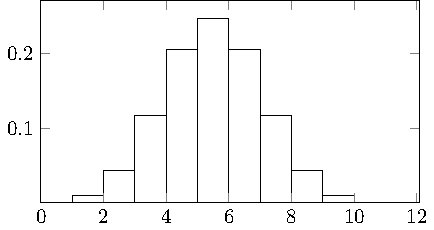
\includegraphics[page = 1]{Tikz.pdf}
    \includegraphics[page = 2]{Tikz.pdf}
    \caption{à esquerda temos a plotagem da densidade de uma $\operatorname{Bin}(10, 0.25)$ em forma de histograma, já à direita a plotagem da acumulada da mesma.}
    \label{gaussianas}
\end{figure}

Note que se traçarmos uma reta $y = \alpha_0$, nem sempre podemos encontrar um valor $k$ de forma que a acumulada da distribuição tenha imagem $\alpha_0$. Como exemplo, se traçarmos a reta $y = 0.2$, como se estivéssemos considerando $\alpha_0 = 0.2$, não temos nenhum ponto $k$ que nos dê um teste de nível $\alpha_0$ no experimento descrito anteriormente. A ideia aqui é que você proponha uma solução para isso, ou seja, mostre como podemos fazer nosso teste de modo que possamos atingir qualquer nível $\alpha_0$ em $(0, 1)$.

\section*{Conclusão}

Em primeiro lugar, pude concluir nas férias que palhaços e bananas pode resultar numa combinação explosiva. Além disso, vi que a frase ``nunca fale com estranhos na rua'' realmente é muito válida.

\begin{comment}
Já no início pudemos ter uma boa ideia do significado da precisão, sendo visualizada como uma métrica de proximidade dos dados em relação a média. Após isso passamos a fazer uma análise bayesiana com a normal com média e precisão desconhecidas. Feita a análise, descobrimos mais uma família conjugada, agora com duas distribuições a priori. Além disso, a visualização de $\lambda_0$ como um nível de certeza a priori acabou deixando o cálculo da média a posteriori, $\mu_1$, um pouco mais intuitivo. Além dele, vimos que $\alpha_0$ e $\beta_0$ são hiperparâmetros que irão contribuir na forma da posteriori de $\mu$, ditando a concentração em torno de $\mu_1$.

Chegando no exemplo vimos que a escolha da priori tem certa relevância no cálculo da posteriori, embora os intervalos de credibilidade que foram gerados ficaram próximos. Além disso, vimos que a medida em que $n$ cresce essa relevância  da priori diminui. Ou seja, a priori pode ser gerada de diversas formas, a depender da interpretação de quem vai elaborá-la, mas a posteriori nos dará resultados similares e, com uma grande amostragem, as posterioris tendem a uma mesma distribuição.

Assim, uma das maiores lições desse trabalho é que elicitar prioris pode ser muito complicado, podendo ser considerada uma arte na qual o ponto de vista e interpretação do artista pode ser crucial para obtermos um resultado razoável ou então um totalmente descartável.

Por fim, talvez seria interessante alguém falar com Palmirinha para ela buscar um assistente menos comilão, imagine ele fazendo uma amostragem de $100$ pamonhas!

\end{comment}

\section*{Resposta do desafio}

O leitor mais atento provavelmente deve ter relacionado o problema com uma nota de rodapé que apareceu na seção ``Teste UMP e MLR''. Essencialmente, a solução do desafio proposto é exatamente aplicar aquela ideia, ou seja, dado um nível $\alpha_0$ se encontrarmos $c$ de forma que
\[P(r(X) \geq c \mid \theta = \theta_0) = \alpha_0,\]

\noindent está perfeito e temos nosso teste pronto, caso contrário, isto é, não existe $c$ que satisfaça a relação acima, podemos encontrar um valor $c$ tal que
\[P(r(X) \geq c \mid \theta = \theta_0) < \alpha_0 \text{ e } P(r(X) \geq c + 1 \mid \theta = \theta_0) > \alpha_0.\]

Agora, se rejeitarmos $H_0$ caso $r(X) \geq c$, o tamanho do teste será menor que $\alpha_0$, mas rejeitando $H_0$ quando $r(X) \geq c + 1$, o tamanho será maior que $\alpha_0$. Nesse caso, a solução é rejeitar $H_0$ se $r(X) \geq c$ e, se $r(X) = c + 1$, rejeitamos $H_0$ com uma probabilidade $q$, a qual será escolhida de forma que
\[q\cdot P(r(X) = c + 1 \mid \theta = \theta_0) + P(r(X) \geq c \mid \theta = \theta_0) = \alpha_0,\]

\noindent onde conseguimos ter um teste de nível $\alpha_0$.

\printbibliography

\end{document}
